\chapter{Anhang}\label{sec:anhang}
\lstset{ % Octave Settings
	language=Octave,
	extendedchars=true,
	basicstyle=\footnotesize,
	numbers=left,
	numberstyle=\tiny\color{gray},
	stepnumber=1,
	numbersep=10pt,
	showspaces=false,
	showstringspaces=false,
	tabsize=2,
	breaklines=true,
	frame=single,
	morecomment = [l][\itshape\color{blue}]{\%},
	captionpos=b,
	title=\lstname
}
\lstinputlisting{data/Aufgabe6_2a.m}
\lstinputlisting{data/SkriptAg6_2.m}

\begin{figure}[h]
	\centering
	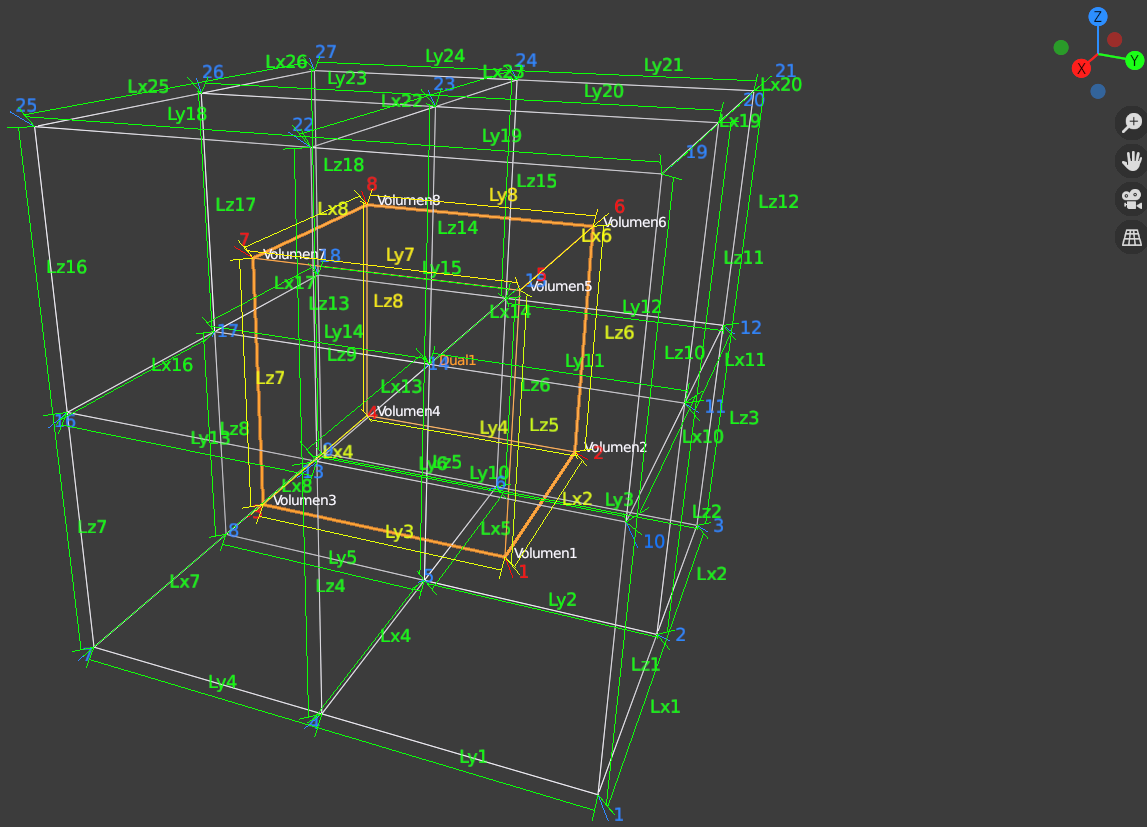
\includegraphics[width=\textwidth]{data/Everything}
	\caption{Vollständig beschriftetes Primales und duales Gitter}
	\label{fig:alles}
\end{figure}


